\PassOptionsToPackage{unicode=true}{hyperref} % options for packages loaded elsewhere
\PassOptionsToPackage{hyphens}{url}
%
\documentclass[ignorenonframetext,]{beamer}
\usepackage{pgfpages}
\setbeamertemplate{caption}[numbered]
\setbeamertemplate{caption label separator}{: }
\setbeamercolor{caption name}{fg=normal text.fg}
\beamertemplatenavigationsymbolsempty
\usepackage{lmodern}
\usepackage{amssymb,amsmath}
\usepackage{ifxetex,ifluatex}
\usepackage{fixltx2e} % provides \textsubscript
\ifnum 0\ifxetex 1\fi\ifluatex 1\fi=0 % if pdftex
  \usepackage[T1]{fontenc}
  \usepackage[utf8]{inputenc}
  \usepackage{textcomp} % provides euro and other symbols
\else % if luatex or xelatex
  \usepackage{unicode-math}
  \defaultfontfeatures{Ligatures=TeX,Scale=MatchLowercase}
\fi
\usetheme[]{metropolis}
% use upquote if available, for straight quotes in verbatim environments
\IfFileExists{upquote.sty}{\usepackage{upquote}}{}
% use microtype if available
\IfFileExists{microtype.sty}{%
\usepackage[]{microtype}
\UseMicrotypeSet[protrusion]{basicmath} % disable protrusion for tt fonts
}{}
\IfFileExists{parskip.sty}{%
\usepackage{parskip}
}{% else
\setlength{\parindent}{0pt}
\setlength{\parskip}{6pt plus 2pt minus 1pt}
}
\usepackage{hyperref}
\hypersetup{
            pdfborder={0 0 0},
            breaklinks=true}
\urlstyle{same}  % don't use monospace font for urls
\newif\ifbibliography
\usepackage{graphicx,grffile}
\makeatletter
\def\maxwidth{\ifdim\Gin@nat@width>\linewidth\linewidth\else\Gin@nat@width\fi}
\def\maxheight{\ifdim\Gin@nat@height>\textheight\textheight\else\Gin@nat@height\fi}
\makeatother
% Scale images if necessary, so that they will not overflow the page
% margins by default, and it is still possible to overwrite the defaults
% using explicit options in \includegraphics[width, height, ...]{}
\setkeys{Gin}{width=\maxwidth,height=\maxheight,keepaspectratio}
% Prevent slide breaks in the middle of a paragraph:
\widowpenalties 1 10000
\raggedbottom
\setbeamertemplate{part page}{
\centering
\begin{beamercolorbox}[sep=16pt,center]{part title}
  \usebeamerfont{part title}\insertpart\par
\end{beamercolorbox}
}
\setbeamertemplate{section page}{
\centering
\begin{beamercolorbox}[sep=12pt,center]{part title}
  \usebeamerfont{section title}\insertsection\par
\end{beamercolorbox}
}
\setbeamertemplate{subsection page}{
\centering
\begin{beamercolorbox}[sep=8pt,center]{part title}
  \usebeamerfont{subsection title}\insertsubsection\par
\end{beamercolorbox}
}
\AtBeginPart{
  \frame{\partpage}
}
\AtBeginSection{
  \ifbibliography
  \else
    \frame{\sectionpage}
  \fi
}
\AtBeginSubsection{
  \frame{\subsectionpage}
}
\setlength{\emergencystretch}{3em}  % prevent overfull lines
\providecommand{\tightlist}{%
  \setlength{\itemsep}{0pt}\setlength{\parskip}{0pt}}
\setcounter{secnumdepth}{0}

% set default figure placement to htbp
\makeatletter
\def\fps@figure{htbp}
\makeatother

\title{Extracting Model Structure for Improved Semantic Modeling}
\date{12/5/2018}
\author{James Fairbanks, Georgia Tech Research Institute}

\begin{document}

\begin{frame}
\maketitle{}
\end{frame}

\begin{frame}{Goals}
\protect\hypertarget{goals}{}

\begin{enumerate}
\tightlist
\item
  Extract a knowledge graph from Scientific Artifacts (code, papers,
  datasets)
\item
  Represent scientific models as a high level abstraction, (code as data)
\item
  Build metamodels by combining models in hierarchical expressions using
  reasoning over KG (1).
\end{enumerate}

\end{frame}

\begin{frame}{Running Example: Influenza}
\protect\hypertarget{running-example-influenza}{}

Modeling the cost of treating a flu season taking into account weather
effects.

\begin{enumerate}
\tightlist
\item
  Seasonal temperature is a dynamical system
\item
  Flu infectiousness is a function of temperature
\end{enumerate}

\end{frame}

\begin{frame}{Running Example: Modeling types}
\protect\hypertarget{running-example-modeling-types}{}

Modeling the cost of treating a flu season taking into account weather
effects.

\begin{enumerate}
\tightlist
\item
  Seasonal temperature is approximated by 2nd order linear ODE
\item
  Flu cases is an SIR model 1st order nonlinear ode
\item
  Mitigation cost is Linear Regression on vaccines and cases
\end{enumerate}

\end{frame}

\begin{frame}{Scientific Domain}
\protect\hypertarget{scientific-domain}{}

We focus on Susceptible Infected Recovered model of epidemiology.

\begin{enumerate}
\tightlist
\item
  Precise, concise mathematical formulation
\item
  Diverse class of models, ODE vs Agent-based, determinstic vs
  stochastic
\item
  FOSS implementations are available in all three Scientific programming
  languages
\end{enumerate}

\end{frame}

\begin{frame}{Graph of SIR Model}
\protect\hypertarget{graph-of-sir-model}{}

\begin{figure}
\centering
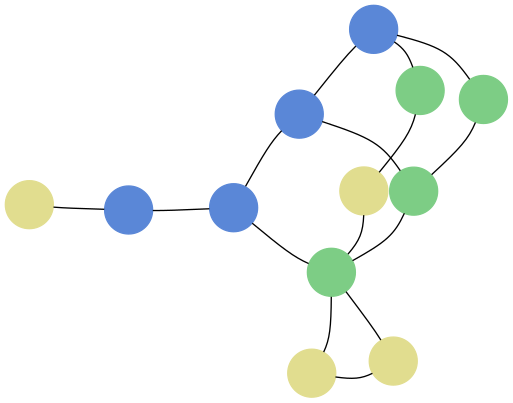
\includegraphics[width=.8\textwidth]{img/sir_graph.dot.png}
\end{figure}

\end{frame}

\begin{frame}{Knowledge Extraction Architecture}
\protect\hypertarget{knowledge-extraction-architecture}{}

\begin{figure}
\centering
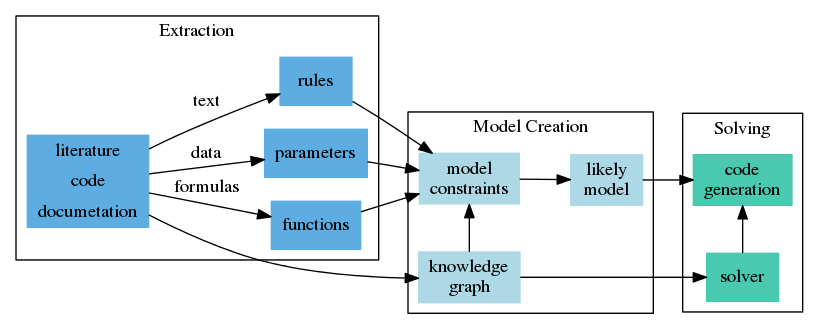
\includegraphics[width=.8\textwidth]{img/extraction.dot.png}
\end{figure}

\end{frame}

\begin{frame}{Example Input Packages}
\protect\hypertarget{example-input-packages}{}

\begin{enumerate}
\tightlist
\item
  EMOD, Epimodels, NetLogo, and FRED are established packages, given
  their maturity and availability of published papers citing these
  packages.
\item
  Pathogen and NDLib are newer packages, we expect easier to work with
  and more future adoption.
\item
  Textbooks~{[}@voit\_first\_2012{]} and lecture notes\footnote<.->{\url{http://alun.math.ncsu.edu/wp-content/uploads/sites/2/2017/01/epidemic_notes.pdf}}
  will be a resource for these simple models that are well
  characterized.
\end{enumerate}

\end{frame}

\begin{frame}{Model Representation and Execution}
\protect\hypertarget{model-representation-and-execution}{}

Representation of models occurs at four levels:

\begin{itemize}
\item
  \textbf{Executable}: the level of machine or byte-code instructions
\item
  \textbf{Lexical}: the tradition code representation assignment,
  functions, and loops
\item
  \textbf{Semantic}: a declarative language or computation graph
  representation with nodes linked to the knowledge graph
\item
  \textbf{Human}: a description in natural language as in a research
  paper or textbook
\end{itemize}

\end{frame}

\begin{frame}{Knowledge Graph Schema}
\protect\hypertarget{knowledge-graph-schema}{}

A preliminary design for types of knowledge in our knowledge graph.
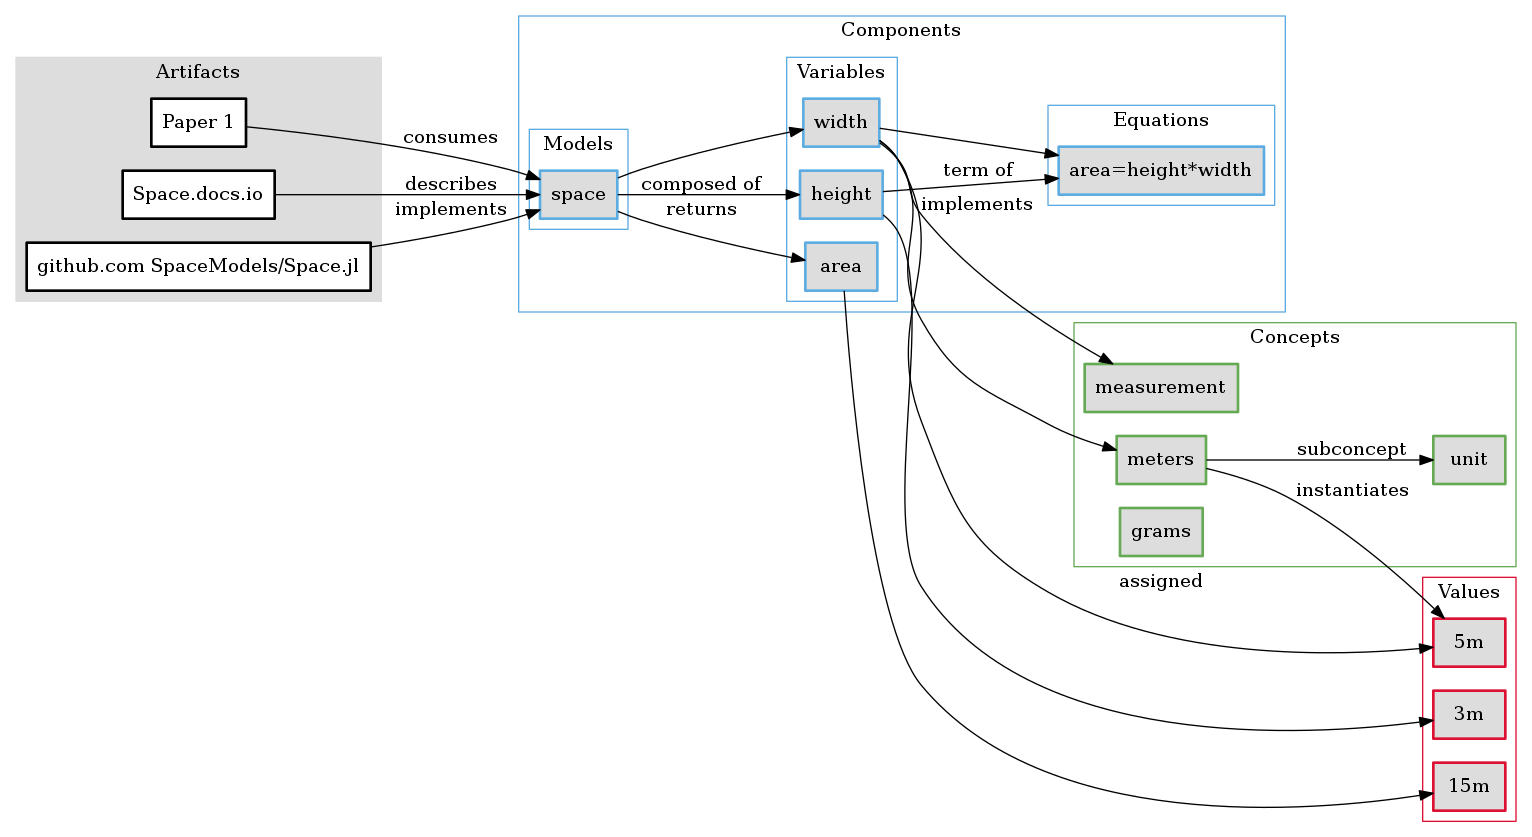
\includegraphics[width=.8\textwidth]{img/schema.dot.png}

\begin{itemize}
\tightlist
\item
  Artifacts
\item
  Components

  \begin{itemize}
  \tightlist
  \item
    Models
  \item
    Variables
  \item
    Equations
  \end{itemize}
\item
  Concepts
\item
  Values
\end{itemize}

\end{frame}

\begin{frame}{Knowledge Graph}
\protect\hypertarget{knowledge-graph}{}

\begin{figure}
\centering
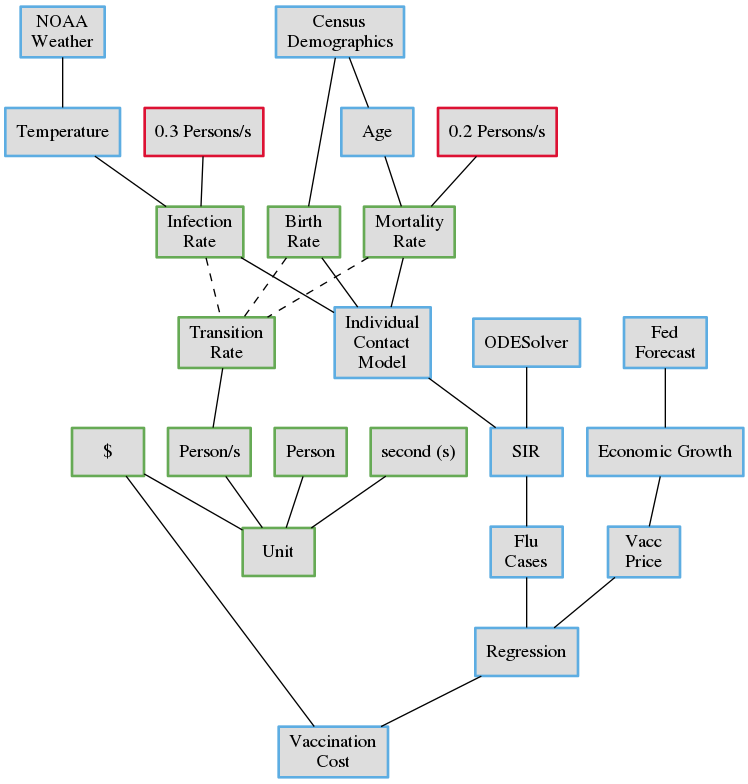
\includegraphics[width=.8\textwidth]{img/knowledgegraph.dot.png}
\caption{Hypothetical Knowledge Graph Sample}
\end{figure}


\end{frame}


\begin{frame}{Flu Metamodel Pipeline}
\protect\hypertarget{flu-metamodel-pipeline}{}

Here is the DAG for our running example.
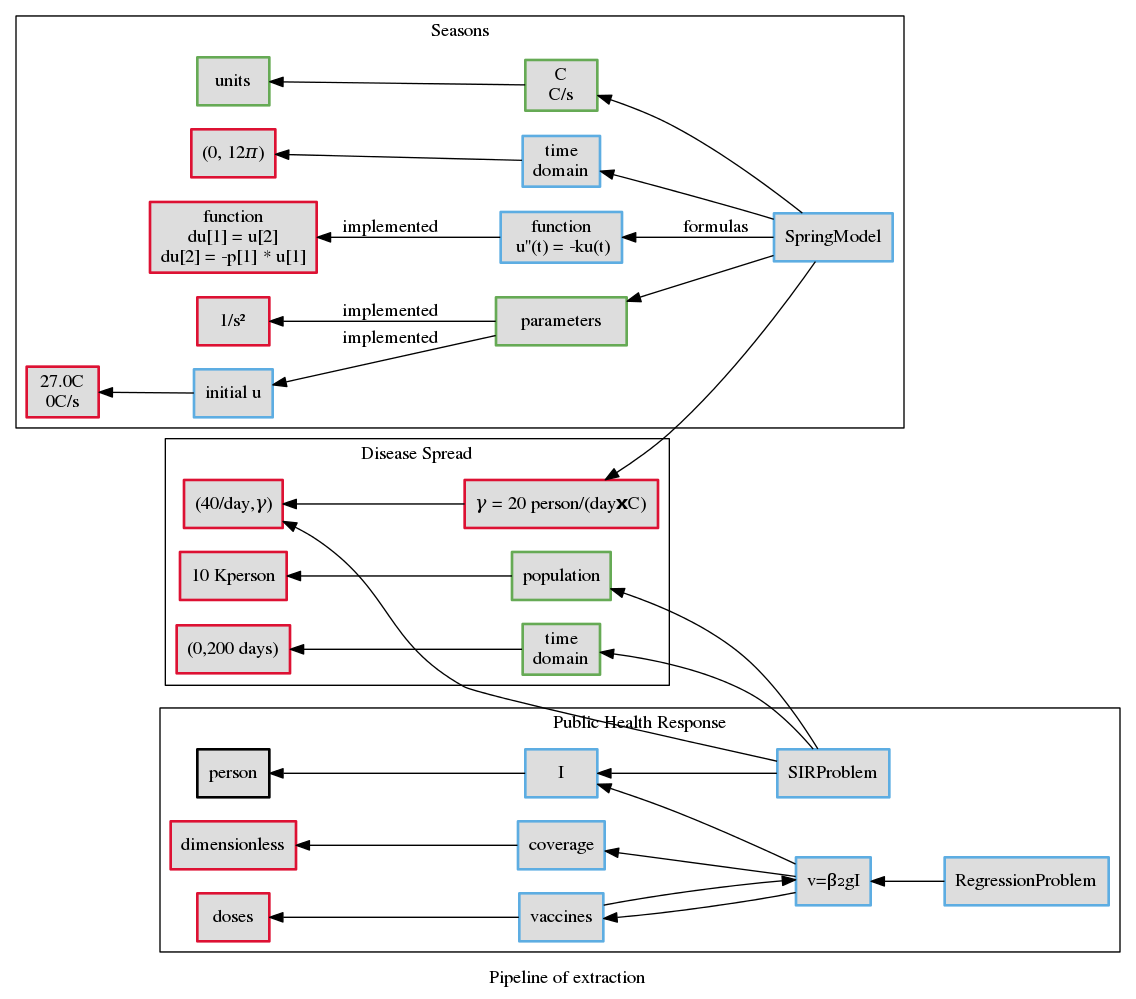
\includegraphics[width=.8\textwidth]{img/flu_pipeline.dot.png}

See \href{@ref}{FluModel} for worked out example.

\end{frame}

\begin{frame}{Knowledge Graph Reasoning}
\protect\hypertarget{knowledge-graph-reasoning}{}

\begin{enumerate}
\tightlist
\item
  Define Model representations / KG schema
\item
  Extract KG from artifacts
\item
  \textbf{Reason over KG to build metamodel}
\item
  CodeGen/Execution of Metamodel
\end{enumerate}

\end{frame}

\begin{frame}{How do we get from Weather to Cost?}
\protect\hypertarget{how-do-we-get-from-weather-to-cost}{}

\begin{figure}
\centering
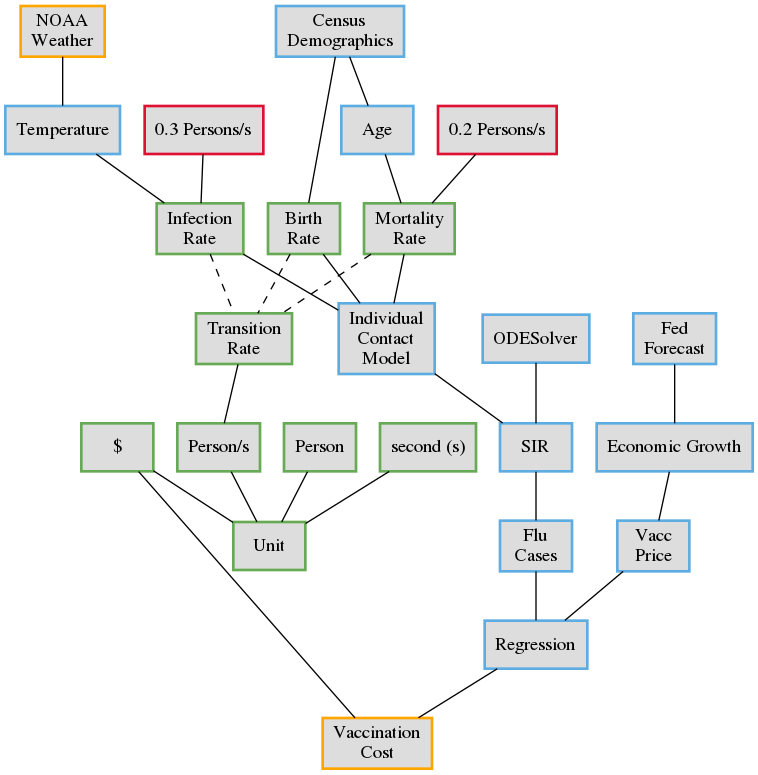
\includegraphics[width=0.8\textwidth,height=0.9\textheight]{img/knowledge_reasoning.dot.png}
\end{figure}

\end{frame}

\begin{frame}{How do we get from Weather+Demographics to Cost?}
\protect\hypertarget{how-do-we-get-from-weatherdemographics-to-cost}{}

\begin{figure}
\centering
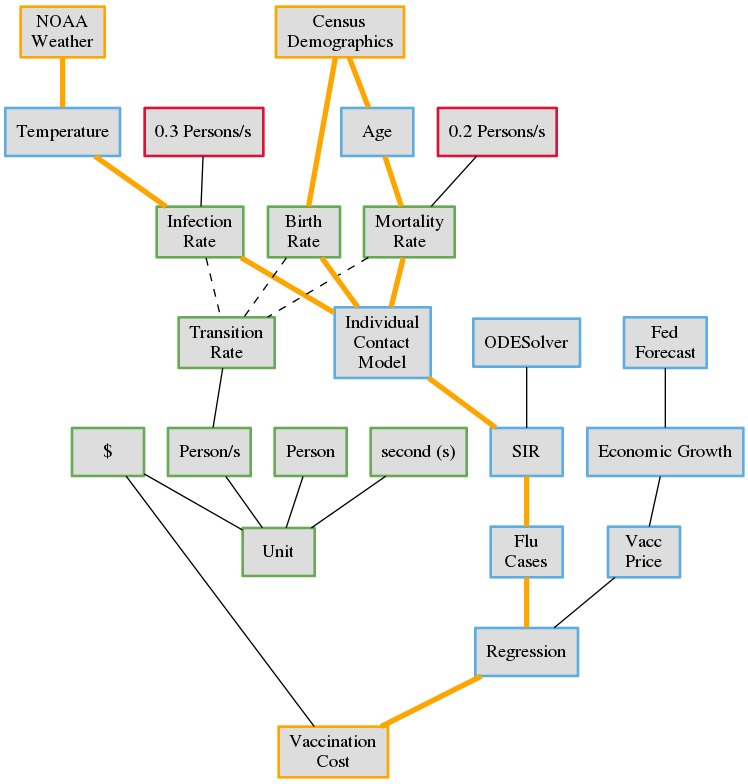
\includegraphics[width=0.8\textwidth,height=0.9\textheight]{img/knowledge_reasoning_flow.dot.png}
\end{figure}

\end{frame}

\begin{frame}{Knowledge Graph Reasoning Open Questions}
\protect\hypertarget{knowledge-graph-reasoning-open-questions}{}

\begin{itemize}
\tightlist
\item
  What rules for path/flow computations are necessary and sufficient for
  a metamodel?
\item
  Can we implement those rules by choosing weights?
\item
  How do we handle uncertainty and near matches?
\item
  How do we determine ``necessary dependencies'' better than ``connected
  component''
\item
  What about supplying expert information?
\end{itemize}

\end{frame}

\begin{frame}{Infectious Disease Metamodel}
\protect\hypertarget{infectious-disease-metamodel}{}

\begin{itemize}
\tightlist
\item
  A more ambitious example of a metamodel
\item
  Requires Agent-based simulations of information diffuision and disease
  spread
\end{itemize}
\begin{figure}
\centering
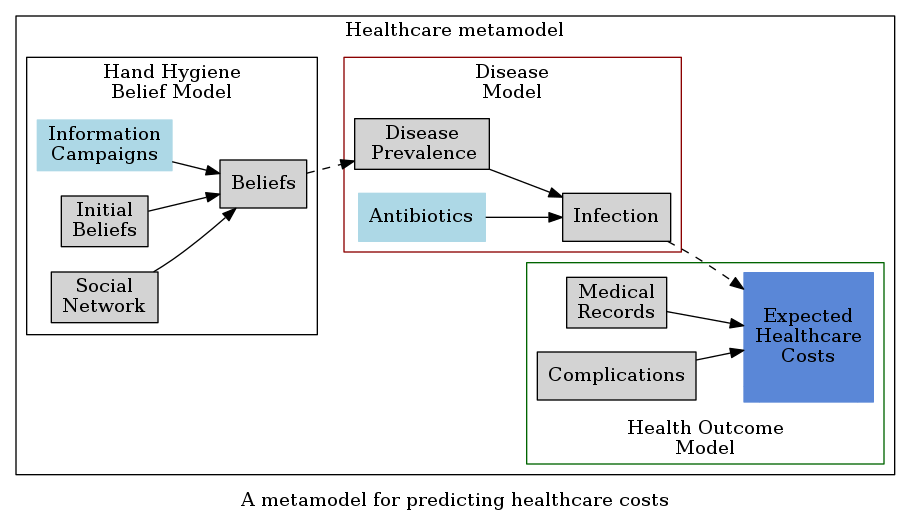
\includegraphics[height=0.7\textheight]{img/metamodel.dot.png}
\caption{A DAG of model dependencies}
\end{figure}

\end{frame}

\begin{frame}{Static vs Dynamic Graph}
\protect\hypertarget{static-vs-dynamic-graph}{}

\begin{itemize}
\tightlist
\item
  Inherent tradeoff between flexibility and static analysis
\item
  We will build the computation graph through the execution of code
\item
  Metaprogramming will be used to generate the executable codes
\end{itemize}

\end{frame}

\begin{frame}{Validation}
\protect\hypertarget{validation}{}

\begin{itemize}
\tightlist
\item
  Extraction of KG elements from artifacts
\item
  Metamodel construction
\item
  Metamodel quality
\end{itemize}

\begin{block}{Error and Residual}

\begin{itemize}
\item
  Analogize the metamodel construction error and the model quality to
  the error and residual in numerical solvers. Given \(f(x)=0\) solve
  for \(x\)
\item
  Measure both the error and the residual.
\item
  Error \(\mid x-x^\star\mid\), the difference from the correct solution
\item
  Residual \(\mid f(x) - f(x^\star)\mid\) or the difference from quality
  of optimal solution
\end{itemize}

\end{block}

\end{frame}

\begin{frame}{Next Steps}
\protect\hypertarget{next-steps}{}

\begin{itemize}
\tightlist
\item
  Incorporation of feedback today

  \begin{itemize}
  \tightlist
  \item
    the types of artifacts in scope
  \item
    domain coverage and desired extensibility
  \item
    inclusion/exclusion of particular package(s) and/or knowledge
    artifact(s)
  \end{itemize}
\item
  Construction of a proof-of-concept version of our knowledge graph and
  end-to-end pipeline
\item
  Tailor running example to DARPA objectives
\item
  A automatic transformation of models at the Semantic Level
\end{itemize}

\end{frame}

\end{document}
